\documentclass[
    % english, % Klasei padavus parametrą 'english', darbas bus anglų kalba.
    % signatureplaces % prideda parašų vietas tituliniame puslapyje
]{VUMIFPSbakalaurinis}
\usepackage{float}
\usepackage{wrapfig2}
\usepackage{hyperref}
\usepackage{algorithmicx}
\usepackage{algorithm}
\usepackage{algpseudocode}
\usepackage{amsfonts}
\usepackage{amsmath}
\usepackage{bm}
\usepackage{caption}
\usepackage{color}
\usepackage{graphicx}
\usepackage{listings}
\usepackage{subcaption}
\usepackage{biblatex}

% Titulinio aprašas
\university{Vilniaus universitetas}
\faculty{Matematikos ir informatikos fakultetas}
\department{Programų sistemų bakalauro studijų programa}
\papertype{Bakalauro baigiamojo darbo planas}
\title{Duomenų augmentacijų efektyvumas nustatant ligas plaučių echoskopijose}
\titleineng{Data augmentations effectiveness in detecting diseases with lung ultrasound}
\author{Justas Baniulis}
% \secondauthor{Vardonis Pavardonis}   % Pridėti antrą autorių
\supervisor{asist. dr. Tomas Plankis}
%\reviewer{}
\date{Vilnius – \the\year}

\bibliography{bibliografija}

\begin{document}
\maketitle

% tyrimo objektas ir aktualumas, 
% darbo tikslas, 
% keliami uždaviniai ir laukiami rezultatai, 
% tyrimo metodai, 
% numatomas darbo atlikimo procesas
% apibūdinami darbui aktualūs literatūros šaltiniai.

% Pastaba. Darbo uždavinyje apibrėžiamas siekiamas rezultatas, kad būtų galimybė išmatuoti,
% ar tikslai ir uždaviniai yra išspręsti, bei kokiu lygiu (vertinant kiekybę bei kokybę). Pavyz-
% džiui, „Atlikti literatūros .... analizę“ nėra tinkamas uždavinys, nes nusako procesą, tačiau
% neapibrėžia jo rezultato. Tinkamos uždavinio formuluotės šablonai: „Išanalizuoti literatūrą
% … siekiant apžvelgti ir įvertinti /… metodų tinkamumą sprendžiamam uždaviniui/privalu-
% mus ir trūkumus sprendžiant … uždavinį/rekomenduojamas ... projektavimo gaires, šablonus
% ir pan.“

\sectionnonum{Darbo planas}
Plaučių echoskopija yra tyrimas atliekamas su echoskopijos įrenginiu, kuris vizualizuoja plaučių organo artefaktus naudodamas aukšto dažnio garso bangas. Sveikatos priežiūros specialistas echoskopuoja paciento krūtinę naudodamasis echoskopijos įrenginiu, kuris realiu laiku skleidžia garso bangas, šios bangos atšoka aptikusios kliūtį ir atšokusios bangos yra surenkamos tame pačiame įrenginyje. Bangos atšoka skirtingai nuo skirtingų medžiagų, kaip oras, skystis, audiniai ir galutiniame echoskopijos rezultate yra išgaunami kadrai, kuriuose sveikatos priežiūros specialistas gali pastebėti garso bangų suformuotus artefaktus, kaip pavaizduotus \ref{img:plauciai_art} paveikslėlyje.
\begin{figure}[H]
    \centering
    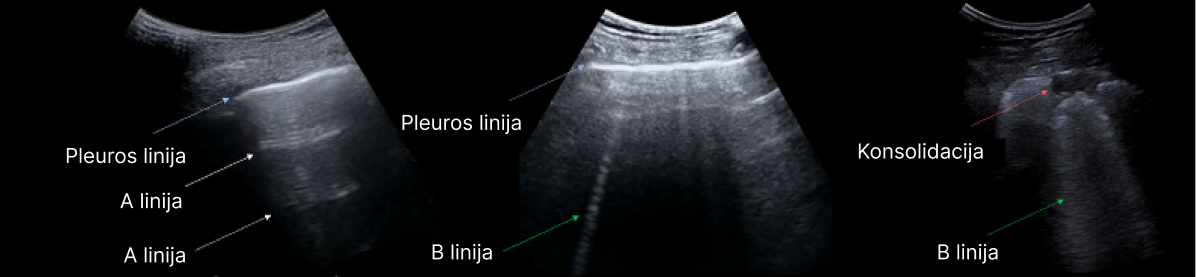
\includegraphics[scale=0.391]{img/plauciai_artefaktai.png}
    \caption{Plaučių artefaktų pavyzdžiai \cite{demi2023new}}
    \label{img:plauciai_art}
\end{figure}
Plaučių echoskopijos tyrime yra interpretuojami artefaktai, kaip A linijos, B linijos, konsolidacijos ir pleuros ertmės (linijos). Naudojantis pastebimais artefaktais, gydytojas gali diagnozuoti ligas ar nustatyti sveikų plaučių diagnozę (žr. \ref{tab:ligos} lentelę). 
\begin{table}[H]\footnotesize
  \centering
  \caption{Echoskopijos artefaktų ir ligų sąryšis \cite{demi2023new, cammarota2023lung}}
  \begin{tabular}{|l|c|c|c|c|c|} \hline
     Artefaktas & Galimos diagnozės \\
    \hline
    A linija  & Sveiki plaučiai \\
    B linija & Širdies ydos, COVID-19, virusinis plaučių uždegimas, plaučių edema \\
    Konsolidacija & Bakterinis plaučių uždegimas, atelektazė, plaučių sumušimas \\
    Pleuros linija & Pneumotoraksas, pleuros efuzija, pleuros fibrozė \\
    \hline
  \end{tabular}
  \label{tab:ligos}
\end{table}
\par
Šis tyrimas paskutinį dešimtmetį yra vis populiarėjantis tarp medikų tiriant plaučius ir nustatant jų diagnozę \cite{demi2023new}. Plaučių echoskopija yra patrauklus tyrimas gydytojams, nes jo kaina mažesnė už įprastai naudojamus rentgeno ar tamografijos tyrimus, kadangi echoskopinė įranga daug pigesnė už radiologinę, paciento nereikia transportuoti į radiologinį skyrių, echoskopijos prietaisai neskleidžia paciento sveikatai pavojingos radiacijos, patyręs medicinos profesionalas gali interpretuoti echoskopiją tiksliau nei rentgeno nuotraukas ir greičiau, nes echoskopijos prietaisai skleidžia, surenka aukšto dažnio bangas ir atgamina artefaktus realiu laiku. Šio tyrimo trūkumas yra tai, kad išmokti teisingai nustatyti artefaktus ir iš jų nustatyti ligos diagnozę interpretuojant echoskopijos rezultatus yra sunku. Taip pat užtrunka laiko ir žmogiškųjų išteklių išmokinti teisingai nustatyti diagnozę \cite{cammarota2023lung}.

% Įvade aprašomi darbo tikslai, 
Specialistams ligos diagnozavimo darbą su plaučių echoskopijos tyrimais gali palengvinti dirbtinis intelektas \cite{demi2023new, born2021accelerating}. 2021 metų straipsnio autoriai pateikia atvirą duomenų rinkinį POCUS (liet. echoskopijos paimtos iš priežiūros vietos), kuriame surinkti medicinos profesionalų suklasifikuotos echoskopinės nuotraukos ir vaizdo įrašai. Pasak autorių, šis atviras naudojimui duomenų rinkinys yra skirtas neuroninų tinklų modeliams treniruoti. Autoriai surinko 4 klasių echoskopijų į vieną rinkinį: COVID-19, bakterinio uždegimo (pneumonijos), virusinio uždegimo ir sveikų plaučių. Duomenų pavyzdžiai pateikti \ref{img:pocus} paveikslėlyje.

\begin{figure}[H]
    \centering
    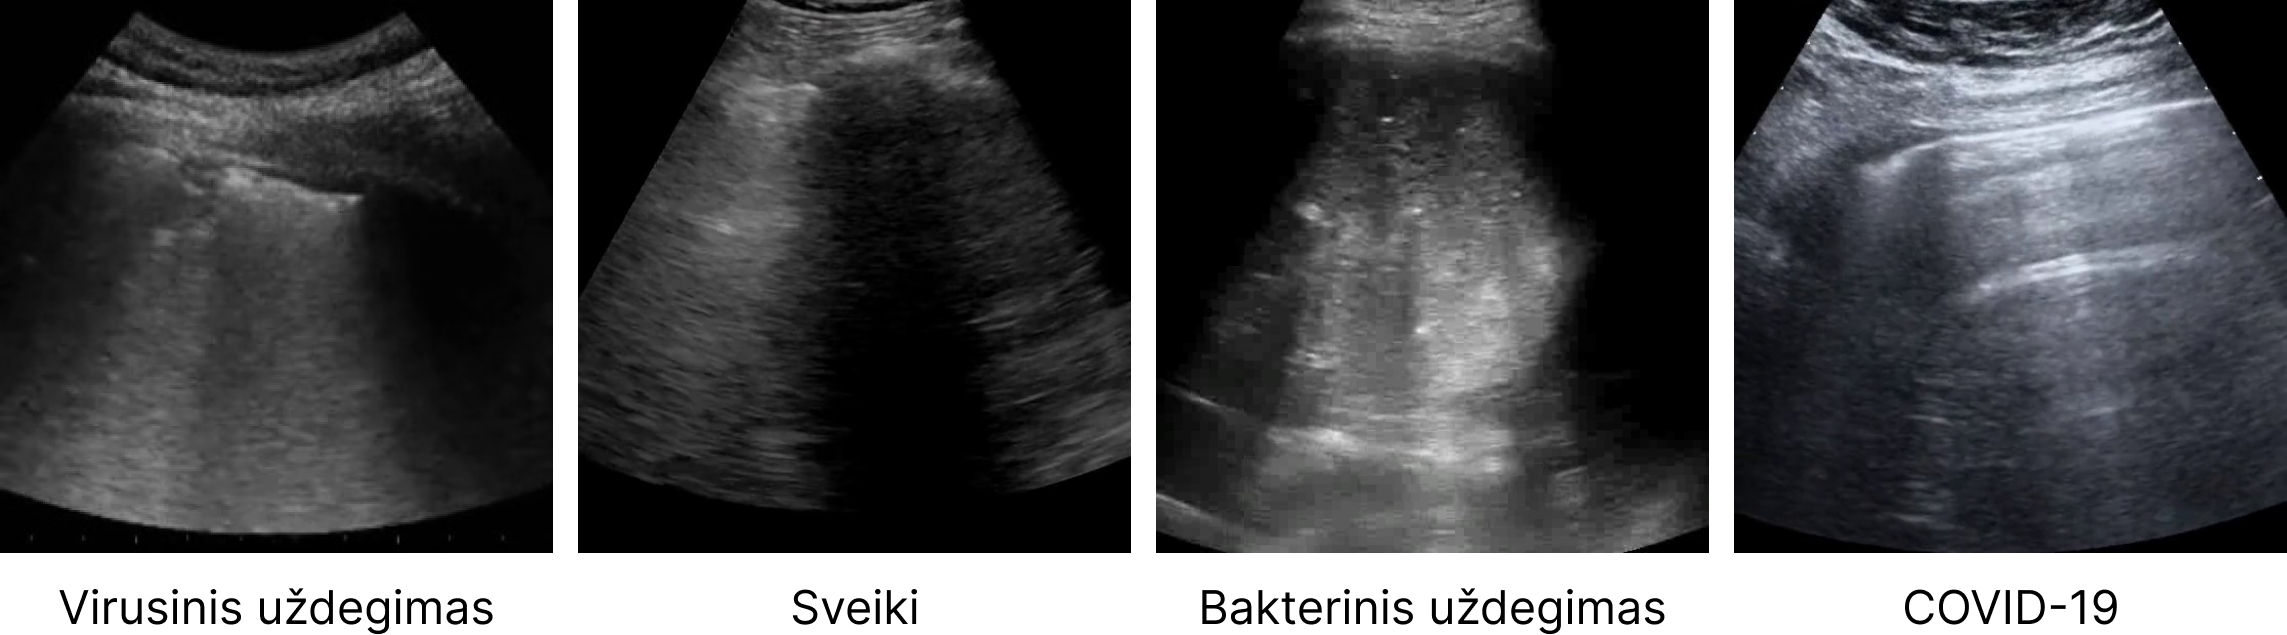
\includegraphics[scale=0.20099]{img/pocus.png}
    \caption{POCUS duomenų rinkinio klasių pavyzdžiai \cite{born2021accelerating}}
    \label{img:pocus}
\end{figure}

\printbibliography[heading=bibintoc]
\end{document}
